\chapter{Histograms}

\section{Introduction}

In this exercise, you will learn how to produce and display
histograms, and compare histogram data with a distribution function.

\section{Histogram of Simulated Data}

First we will generate fake data, called Monte Carlo data, in order to
have something to plot.  We'll use the {\tt random.norm} function to
produce 200 events randomly drawn from a Gaussian distribution with
mean of 5, and sigma of 1.5:
\begin{center}
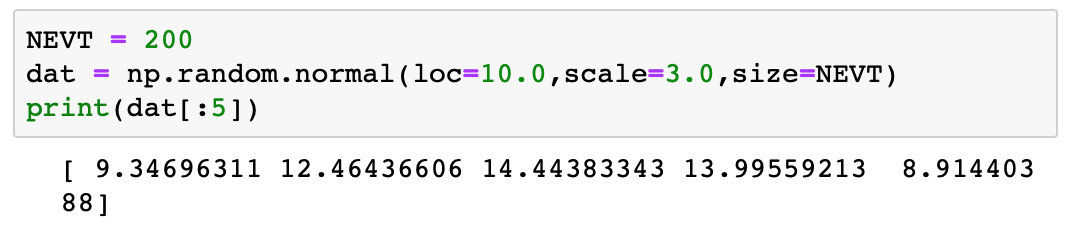
\includegraphics[width=0.85\textwidth]{figs/histograms/mc.png}\\ 
\end{center}
Notice the scipy names for the Gaussian parameters are {\tt loc} for
the mean, and {\tt scale} for $\sigma$.  The first five events of the
200 produced are printed to the screen as a quick check of our work.

\begin{figure}[htbp]
\begin{center}
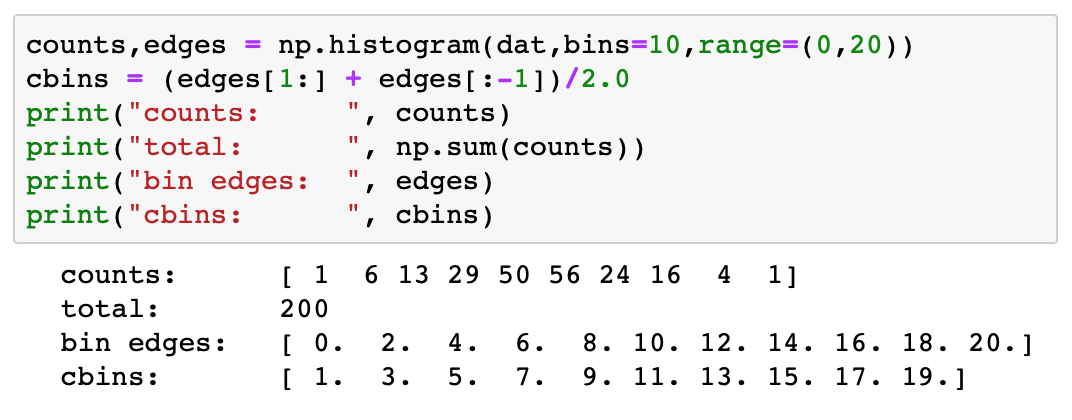
\includegraphics[width=0.85\textwidth]{figs/histograms/hist.png} 
\end{center}
\caption{\label{fig:hist} Example creating a histogram.}
\end{figure}

Next we'll produce a histogram for this simulated data, as shown in
Fig.~\ref{fig:hist} using the scipy {\tt histogram} function:
\begin{verbatim}
counts,edges = np.histogram(dat,bins=10,range=(0,20))
\end{verbatim}
where we have specified 10 bins, uniformly covering the range from 0
to 20.  The function returns to arrays, which we save as {\tt counts}
and {\tt edges}.  The {\tt counts} array contains the bin contents,
the count of the number of values in each bin:
\begin{verbatim}
counts:      [ 1  6 13 29 50 56 24 16  4  1]
\end{verbatim}
The edges array contains the edges of the bins:
\begin{verbatim}
bin edges:   [ 0.  2.  4.  6.  8. 10. 12. 14. 16. 18. 20.]
\end{verbatim}
You'll notice that 10 consecutive bins have 11 edges.  When plotting continuous data, plot the contents at the center of each bin:
\begin{verbatim}
cbins = (edges[:-1] + edges[1:])/2.0
\end{verbatim}
Here the two slices {\tt edges[:-1]} and {\tt edges[1:]} are all but the last and all but the first edges.  The average of the two is the center of each bin:
\begin{verbatim}
cbins:    [ 1.  3.  5.  7.  9. 11. 13. 15. 17. 19.]
\end{verbatim}

We can take a quick look at the histogram data with the {\tt plot} function:
\begin{center}
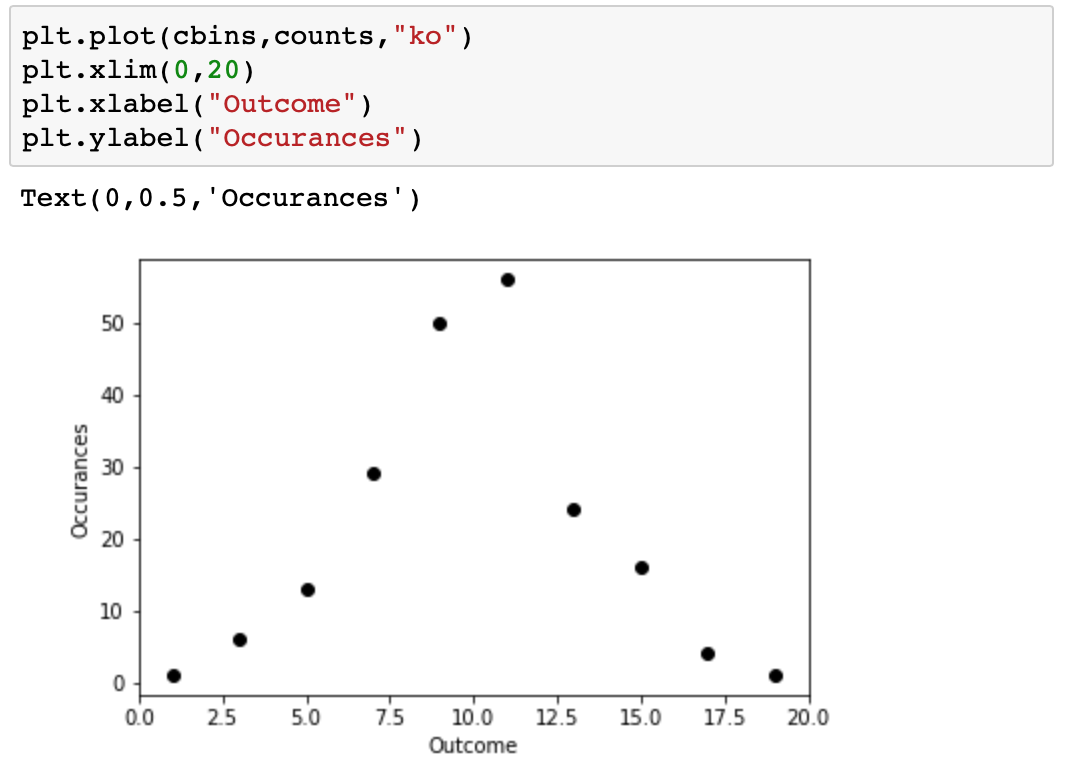
\includegraphics[width=0.85\textwidth]{figs/histograms/plot.png}\\ 
\end{center}

The content of each bin is a single number, a count, and is therefore
subject to the Poisson distribution.  We can estimate the mean of the
Poisson distribution by the measured value, so that $\lambda = N$.
For the Poisson distribution, the variance $\sigma^2 = \lambda$, and
so $\sigma = \sqrt{N}$.  It is customary to draw a line of size
$\sqrt{N}$ when plotting a histogram value $N$. This is an example of
an error bar, which indicates how well our measurement has determined
a particular value.
\begin{center}
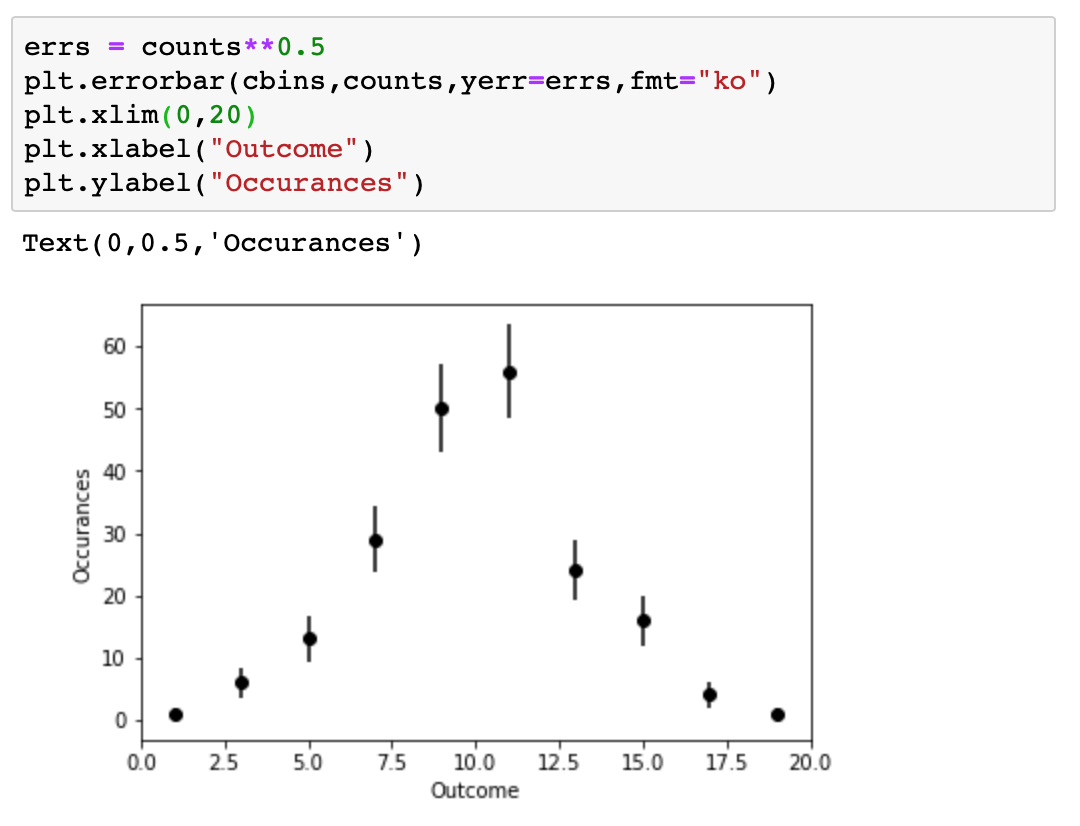
\includegraphics[width=0.85\textwidth]{figs/histograms/err.png}\\ 
\end{center}

\section{Comparison to Distribution Function}

\begin{figure}[htbp]
\begin{center}
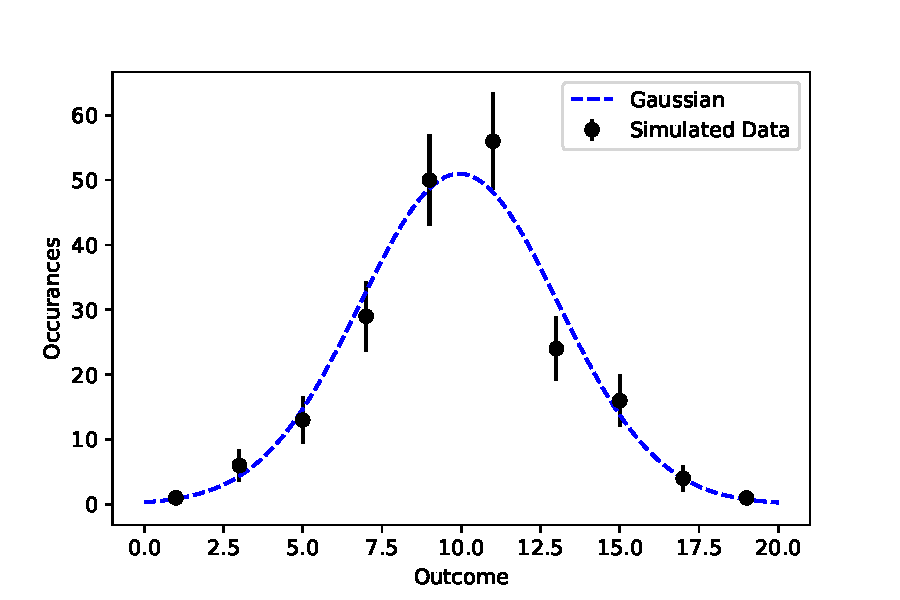
\includegraphics[width=0.7\textwidth]{figs/histograms/gaussian_eg.pdf} 
\end{center}
\caption{\label{fig:gauss} Comparison of simulated data to Guassian PDF.}
\end{figure}

Our theoretical models often predict a PDF for some observable
variable $x$.  As experimentalists, we are often therefore concerned
with the question as to whether our collected data for an observable
$x$ is consistent with the theoretical PDF.  A visual approach to
answering this question is to plot the data in a histogram, and to
draw the PDF as a curve normalized to the histogram.

To predict the number of events in a bin with edges $x_{\rm lower}$
and $x_{\rm upper}$, in principle we need to integrate the PDF and
normalize to the number of experiments:
\begin{displaymath}
N_{\rm pred} = N_{\rm meas} \int^{x_{\rm upper}}_{x_{\rm lower}} p(x) \, dx
\end{displaymath}
In practice, we generally choose the bin sizes small enough that the
PDF is approximately constant during the entire bin, and in this case,
the prediction can be taken as:
\begin{displaymath}
N_{\rm pred} = N_{\rm meas} \; \Delta x \; p(x)
\end{displaymath}
where $\Delta x$ is the width of each bin.  This scale factor $N_{\rm
  meas} \; \Delta x$ allows us to compare a continuous function to
data accumulated within bins.

{\bf Plot 1:} Reproduce the plot in Fig.~\ref{fig:gauss} by comparing
the simulated data to the Gaussian distribution function available
from the {stats.norm.pdf} function.  To use the {\tt stats} library, you will need to import it:
\begin{verbatim}
from scipy import stats
\end{verbatim}
You'll need to appropriately scale the PDF.


{\bf Plot 2:}  Repeat the plot with 10,000 events and 50 bins in the range from $(0,20)$.















